\documentclass[12pt]{article}
\usepackage{amsmath,amssymb,bookmark,graphicx,parskip,textcomp,custom}
\usepackage[margin=.8in]{geometry}
\allowdisplaybreaks
\hypersetup{colorlinks,
    citecolor=black,
    filecolor=black,
    linkcolor=black,
    urlcolor=black
}
\setcounter{secnumdepth}{5}

\begin{document}

\title{SE 464 --- Lab 1}
\author{Kevin Carruthers (20463098)}
\date{\vspace{-2ex}Fall 2015}
\maketitle\HRule

\section{Question 1 -- Interpreter Design}
\begin{figure}[ht]
\centering
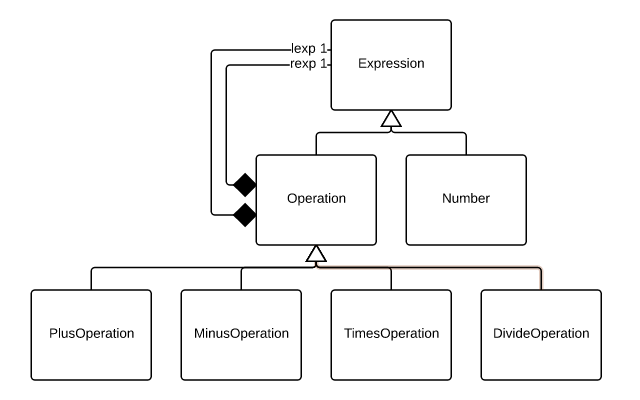
\includegraphics[width=0.8\textwidth]{lab1interpreter.png}
\end{figure}

\newpage

\section{Question 2 -- Visitor Design}
\begin{figure}[ht]
\centering
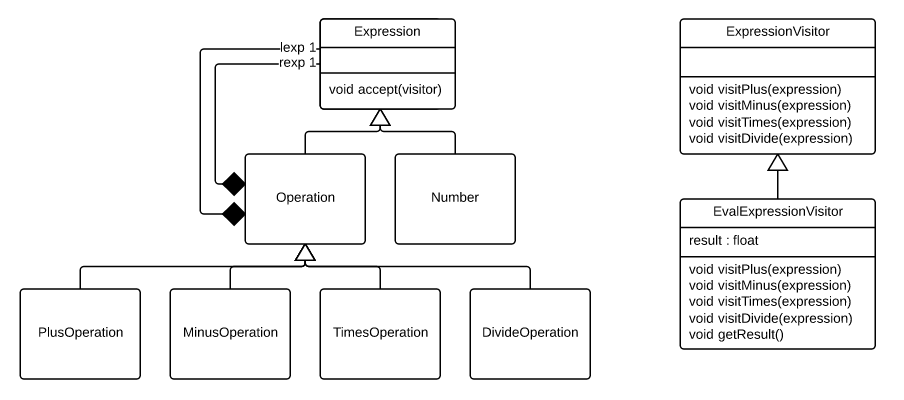
\includegraphics[width=0.8\textwidth]{lab1visitor.png}
\end{figure}

\section{Question 3 -- Out-of-the-Box Design}
RPN could be implemented as a stack; ex. when a user enters ``3 4 +'', we would push ``3'', ``4'', then ``+'' onto the stack. Our process could pop then off in the opposite order (ie. FILO) and curry as it goes, creating an addition function, then partially applying ``3'' to that function, then applying ``4'' to the function and pushing that onto the stack. When we are left with a single value on the stack (in this case, ``7''), our evaluation is complete.

\section{Question 4 -- ``Cheating'' Design}
We could cheat by using a language with an \code{eval} function, such as Python. By calling \code{eval(user\_input)} we could let the interpretor do all the work. Note that this is incredibly vulnerable to malicious input and is a Bad Idea\texttrademark.

\section{Question 5 -- Analysis}
\begin{description}
\item[Part A -- Fitness for Purpose.] All of these designs fulfil the basic functionality requirements.
\item[Part B -- Production Cost.] The first two require a moderate amount of work and knowledge of the respective design patterns. Note the visitor pattern requires slightly more work here as it requires an additional two classes. The latter two methods are far simpler, with the RPN technique being the more complex of the two, albeit safer.
\item[Part C -- Fitness for Future (Factorial).] This requires no work for \code{eval} if the language supports a factorial operator (and is impossible if it does not), requires only an operator definition for RPN, and would require complete overhaul of both the interpretor and visitor patterns to allow for unary operators.
\item[Part D -- Fitness for Future (Printing).] For \code{eval}, interpreter, and visitor, this change would be trivial: the addition of a \code{PrettyPrinter} class which is, in the case of the \code{eval} function, called immediately on the user input or, in the other cases, called on the completed parse tree. For RPN, this class would require a bit more complexity; since it would be reading the values off the stack, it would need to understand RPN-to-standard-format conversion, perform these as it reads through the stack, then place all elements back on the stack in the same order.
\item[Part E -- Design Structure.] These patterns also use composition; which offers a form of multiple inheritance. This pattern can require a lot of boilerplate code.
\end{description}

\end{document}
